\section{Results}
\paragraph{Modeling Allele Frequency Trajectories in Small Populations.} 
We first tested the goodness of fit of the discrete versus Brownian motion (a 
continuous-state model) in modeling allele frequency trajectories, under 
general E\&R
parameters.  For this purpose, we conducted $100$K simulations with
two time samples $\Tc=\{0,\tau\}$ where $\tau\in \{1,10,100\}$ is the
parameter controlling the density of sampling in time.  In addition,
we repeated simulations for different values of starting frequency
$\nu_0\in\{0.005,0.1\}$ (i.e., hard and soft sweep) and selection
strength $s\in\{0,0.1\}$ (i.e., neutral and selection). Then, given
initial frequency $\nu_0$, we computed the expected distribution of
the frequency of the next sample $\nu_\tau$ under two models to make a
comparison.  \ref{fig:markov}A-F shows that Brownian motion
(continuous model) is inadequate when $\nu_0$ is far from $0.5$, or
when sampling times are sparse ($\tau>1$). If the favored allele
arises from standing variation in a neutral population, it is unlikely
to have frequency close to $0.5$, and the starting frequencies are
usually much smaller (see \ref{fig:sfs}). Moreover, in typical \dmel
experiments for example, sampling is sparse. Often, the experiment is
designed so that $10\le\tau\le100$~\cite{kofler2013guide,
  orozco2012adaptation, zhou2011experimental,franssen2015patterns}.

% XXX Not sufficient to say 'in contrast to brownian motion, markov...
% Please check the rewrite of this part
In contrast to the Brownian motion approximation, discrete Markov
chain predictions (Eq.~\ref{eq:Qt}) are highly consistent with
empirical data for a wide range of simulation parameters
(\ref{fig:markov}A-M). Moreover, the discrete markov chain can be
modified to model the case when the the allele is under
selection. 

\begin{figure*}
	\centering
	\includegraphics[width=\textwidth]{{markovDists}.pdf}
	\caption{{\bf Comparison of empirical distributions of allele
			frequencies (red) versus predictions from Brownian
			Motion (green), and Markov chain (blue).}\\
		Comparison of empirical and theoretical distributions under
		neutral evolution (panels A-F) and selection (panels G-M)
		with different starting frequencies $\nu_0\in\{0.005,0.1\}$
		and sampling times of $\Tc=\{0,\tau\}$, where $\tau \in
		\{1,10,100\}$ and $N=1000	$.  For each panel, the empirical 
		distribution
		was computed over 100,000 simulations.  Brownian motion
		(Gaussian approximation) provides poor approximations when
		initial frequency is far from 0.5 (A) or sampling is sparse
		(B,C,E,F). In addition, Brownian motion can only provide
		approximations under neutral evolution. In contrast, Markov
		chain consistently provides a good approximation in all
		cases.}
	\label{fig:markov}
\end{figure*}

\paragraph{Detection Power.} 
We compared the performance of \comale\ against other methods for
detecting selection. For each method we calculated detection power as
the percentage of true-positives identified with false-positive rate
$\le 0.05$. For each configuration (specified with values for
selection coefficient $s$, starting allele frequency $\nu_0$ and
coverage $\lambda$), power of each method is evaluated over $2000$
distinct simulations, half of which modeled neutral evolution and the
rest modeled positive selection.



We compared the power of \comale\ with Gaussian process
(GP)~\cite{Terhorst2015Multi}, FIT~\cite{feder2014Identifying}, and
CMH~\cite{agresti2011categorical} statistics.  FIT and GP convert read
counts to allele frequencies prior to computing the test statistic.
\comale\ shows the highest power in all cases and the power stays
relatively high even for low coverage (\ref{fig:power} and
\ref{tab:power}). In particular, the difference in performance of
\comale\ with other methods is pronounced when starting frequency is
low.  The advantage of \comale\ stems from the fact that favored
allele with low starting frequency might be missed by low coverage
sequencing. In this case, incorporating the signal from linked sites
becomes increasingly important. We note that methods using only two
time points, such as CMH, do relatively well for high selection values
and high coverage. However, the use of time-series data can increase
detection power in low coverage experiments or when starting frequency
is low. Moreover, time-series data provide means for estimating
selection parameters $s,h$ (see below). Finally, as \comale\ is robust
to change of coverage, our results (\ref{fig:power}B,C) suggest that
taking many samples with lower coverage is preferable to sparse
sampling with higher coverage. For comparison purposes, we also tested
\comale\ using the single locus statistic ($L=1$). For the most part,
\comale\ showed an improvement over other methods even with $L=1$, or
showed similar performance. The performance improved with higher $L$.


\begin{figure*}
	\centering
	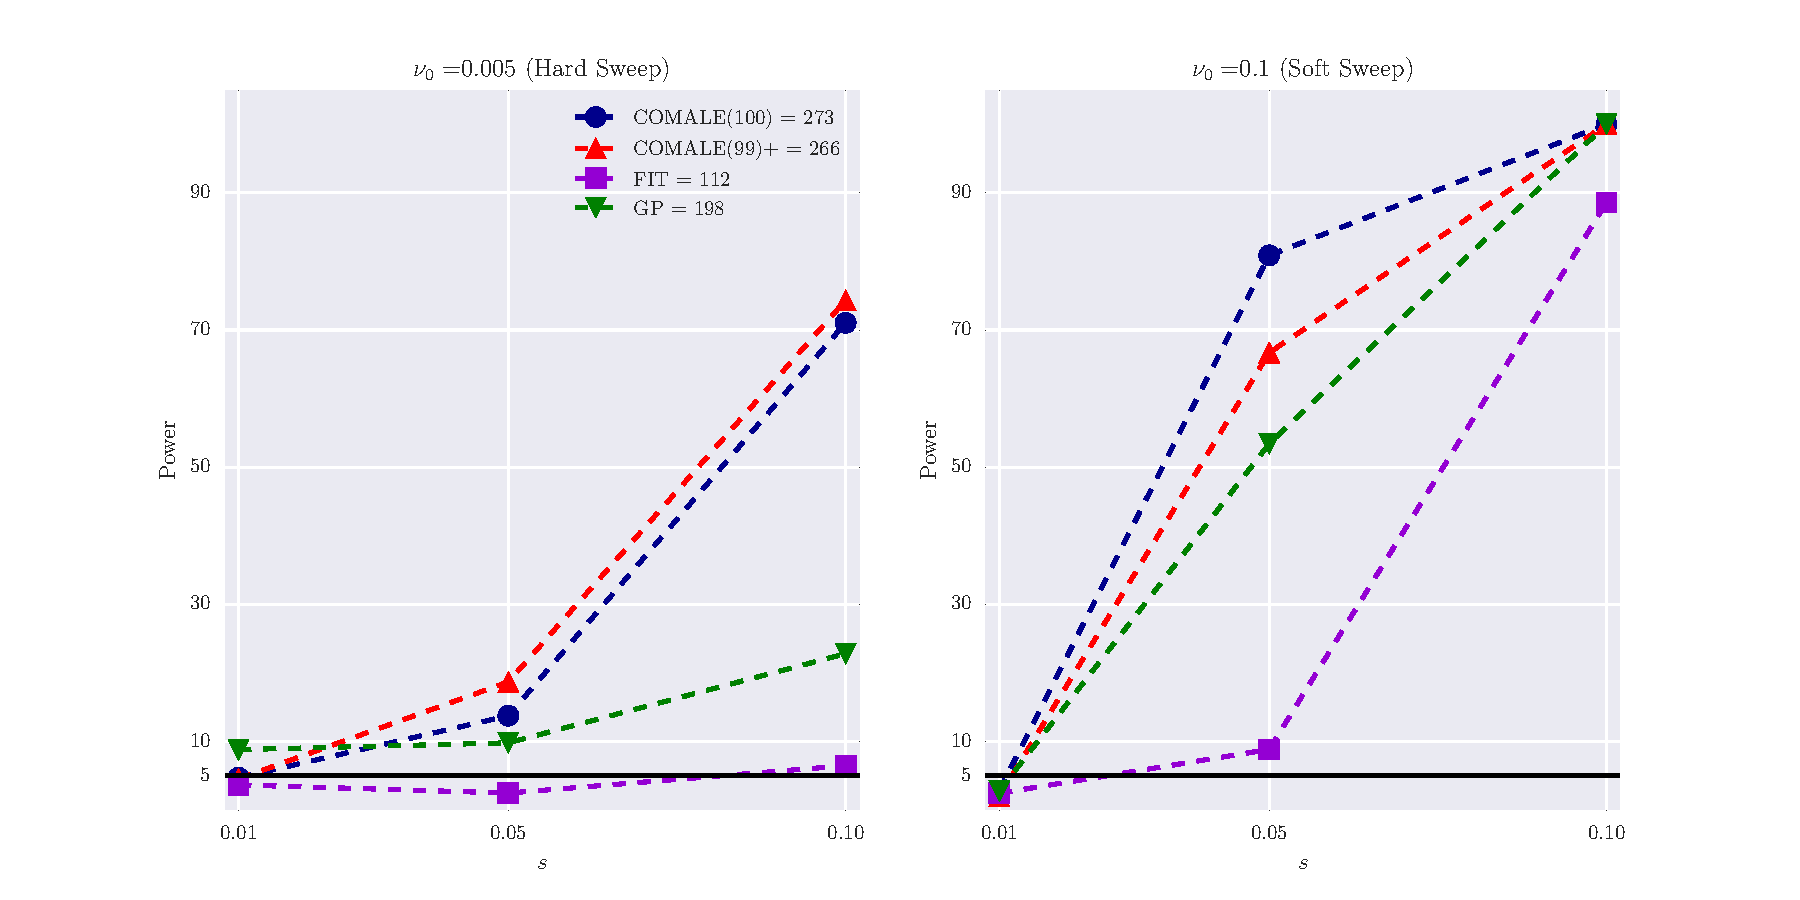
\includegraphics[width=\textwidth]{power.pdf}
	\caption{ {\bf Power calculations for detection of selection.}\\
		Detection power for \comale ($\Hc$), Frequency Increment
		Test (FIT), Gaussian Process (GP), and CMH under hard (A-C)
		and soft sweep (D-F) scenarios. $\lambda$, $s$ denote the
		mean coverage and selection coefficient, respectively.
		Orange hexagons represent the performance of \comale\ when
		the maximum of the single-locus statistic is used to make a
		decision for the genomic region, while the red circle
		corresponds to the performance of \comale\ when single locus
		statistics are averaged over the region.  The $y$-axis
		measures power -- sensitivity with false positive rate FPR
		$\le 0.05$ -- for $2,000$ simulations with $N=1,000$,
		$L=50$Kbp. The horizontal line reflects the power of a
		random classifier.  In all simulations, 3 replicates are
		evolved and sampled at generations
		$\Tc=\{0,10,20,30,40,50\}$.}
	\label{fig:power}
\end{figure*}
\paragraph{Site-identification.}
In general, localizing the favored variant, using pool-seq data is a
nontrivial task due to extensive linkage
disequilibrium~\cite{tobler2014massive}.  To measure performance, we
sorted variants by their $H$ scores and computed rank of the favored
allele for each method. For each setting of $\nu_0$ and $s$, we
conducted $1000$ simulations and computed the rank of the favored
mutation in each simulation. The cumulative distribution of the rank
of the favored allele in 1000 simulation for each setting
(\ref{fig:rank}) shows that \comale\ outperforms other statistics.

An interesting observation is revisiting the contrast between
site-identification and
detection~\cite{long2013massive,tobler2014massive}.  When selection
strength is high, detection is easier (\ref{fig:power}A-F), but
site-identification is harder, due to the high LD between flanking
variants and the favored allele (\ref{fig:rank}A-F).  Moreover,
site-identification becomes more difficult whenever the initial
frequency of the favored allele is low, i.e., at the onset of
selection, LD between favored allele and its nearby variants is
high. For example, when coverage $\lambda=100$ and selection
coefficient $s=0.1$, the detection power is 75\% for hard sweep, but
100\% for soft sweep (\ref{fig:power}B-E). In contrast, the favored
site was ranked as the top in 14\% of hard sweep cases, compared to
and 95\% of soft sweep simulations. 


\begin{figure*}
	\centering
	\includegraphics[trim=.2in 0 .2in 0, 
	clip,width=\textwidth]{{rank100.0}.pdf}
	\caption{{\bf Ranking performance for 100$\times$ coverage.}\\
		Cumulative Distribution Function (CDF) of the distribution
		of the rank of the favored allele in 1000 simulations for
		\comale\ ($H$), Gaussian Process (GP), CMH, and Frequency
		Increment Test (FIT), for different values of selection
		coefficient $s$ and initial carrier frequency. Note that the
		individual variant \comale\ score ($H$) is used to rank
		variants.  The Area Under Curve (AUC) is computed as an overall
		quantitative measure to compare the performance of methods
		for each configuration. In all simulations, 3 replicates with $N=1000$ 
		are evolved and 
		sampled at generations 
		$\Tc=\{0,10,20,30,40,50\}$.}
	\label{fig:rank}
\end{figure*}


\paragraph{Estimating Parameters.}
\comale\ estimates effective population size $\hN$ and selection
parameters, $\hat{s}$ and $\hat{h}$, as a byproduct of the hypothesis
testing. We computed bias of selection fitness ($s-\hat{s}$) and
dominance ($h-\hat{h}$) for of \comale\ and GP for 1000 simulations in
each setting. The distribution of the error (bias) for 100$\times$
coverage is presented in \ref{fig:bias100} for different
configurations.  \ref{fig:bias30} and \ref{fig:biasinf} provide the
distribution of estimation errors for 30$\times$, and 300$\times$
coverage, respectively.  For hard sweep, \comale\ provides estimates
of $s$ with lower variance of bias (\ref{fig:bias100}A and
\ref{fig:biasNull}). In soft sweep, GP and \comale\ both provide unbiased
estimates of $s$ with low variance
(\ref{fig:bias100}B). \ref{fig:bias100}~C-D shows that \comale\
provides unbiased estimates of $h$ as well when $h\in\{0,0.5,1,2\}$
and $s=0.1$.  We also tested if \comale\ provide unbiased estimates of
$N$, by estimating population size on 1000 simulations when $N\in
\{200,600,1000\}$. As shown in~\ref{fig:estimateNMLE}-A 
and~\ref{fig:estimateN}A-C, maximum
likelihood is attained at true value of the parameter.


\begin{figure*}
	\centering
	\includegraphics[width=0.7\textwidth]{{bias.100}.pdf}
	\caption{{\bf Distribution of bias for 100$\times$ coverage.}\\ The
		distribution of bias ($s-\hat{s}$) in estimating selection
		coefficient over 1000 simulations using Gaussian Process (GP) and
		\comale\ ($H$) is shown for a range of choices for the selection
		coefficient $s$ and starting carrier frequency $\nu_0$, when
		coverage $\lambda=100$ (Panels A,B). GP and \comale\ have similar
		variance in estimates of $s$ for soft sweep, while \comale\ provides
		lower variance in hard sweep. Also see \ref{tab:biasdist}. Panels C,D
		show the variance in the estimation of $h$. 
		In all simulations, 3 replicates are evolved and sampled at generations 
		$\Tc=\{0,10,20,30,40,50\}$.}
	\label{fig:bias100}
\end{figure*}

\paragraph{Running Time.}
As \comale\ does not compute exact likelihood of a region (i.e., does
not explicitly model linkage between sites), the complexity of
scanning a genome is linear in number of polymorphisms.  Calculating
score of each variant requires and $\Oc(TRN^3)$ computation
for $\Hc$. However, most of the operations
are can be vectorized for all replicates to make the effective running
time for each variant.  We
conducted $1000$ simulations and measured running times for computing site 
statistics $H$, FIT, CMH and GP with different number of linked-loci.  Our
analysis reveals (\ref{fig:runTime}) that \comale\ is orders of
magnitude faster than GP, and comparable to FIT. While slower than CMH
on the time per variant, the actual running times are comparable after
vectorization and broadcasting over variants (see below).

These times can have a practical consequence. For instance, to run GP
in the single locus mode on the entire pool-seq data of the \dmel genome from a
small sample ($\approx$1.6M variant sites), it would take 1444 CPU-hours
($\approx$ 1 CPU-month). In contrast, after vectorizing and
broadcasting operations for all variants operations using
\texttt{numba} package, \comale\ took 75 minutes to perform an
scan, including precomputation, while the fastest method, CMH, took 17 minutes.

\begin{figure*}
	\centering
	\includegraphics[width=0.75\textwidth]{{runTime.pdf}}
	\caption{{\bf Running time.}\\ Box plots of running time per
		variant (CPU-secs.) of \comale ($\Hc$), CMH, FIT, and
		GP with single, 3, 5, 7, and 10 loci over 1000 simulations
		conducted on a workstation with Intel Core i7
		processor. The average running time for each method is shown
		on the x-axis.
		In all simulations, 3 replicates are evolved and sampled at generations 
		$\Tc=\{0,10,20,30,40,50\}$.}
	\label{fig:runTime}
\end{figure*}


\subsection{Analysis of a \dmel Adaptation to Alternating 
Temperatures}\label{sec:dmel}
We applied \comale\ to the 
\datadm~\cite{orozco2012adaptation,franssen2015patterns}, where
3 replicate samples were chosen from a population of \dmel for 59
generations under alternating 12-hour cycles of  hot stressful (28$^{\circ}$C)
and non-stressful (18$^{\circ}$C) temperatures and sequenced.  In this dataset,
sequencing coverage is different across replicates and generations
(see S2 Fig of~\cite{Terhorst2015Multi}) which makes variant depths
highly heterogeneous (\ref{fig:depthHetero}). 

We first filtered out heterochromatic, centromeric and telomeric
regions~\cite{fiston2010drosophila}, and those variants that have
collective coverage of more that 1500 in all 13 populations: three
replicates at the base population, two replicates at generation 15,
one replicate at generation 23, one replicate at generation 27, three
replicates at generation 37 and three replicates at generation
59. After filtering, we ended up with 1,605,714 variants.

Next, we estimated genome-wide population size $\hN=250$
(\ref{fig:estimateNMLE}-B and \ref{fig:estimateN}-E) which is consistent with 
previous
studies~\cite{orozco2012adaptation,jonas2016estimating}. The
likelihood curves of \comale\ are sharper around the optimum compared
to that of Bollback et. al~\cite{bollback2008estimation}'s method (see
Supplementary Fig. 1 in~\cite{orozco2012adaptation}).  Also,
chromosomes 3L and 3R appear to have smaller population
size, $\hN=200,150$, respectively. 
Others have
made similar observations on this data. In particular,
J\'{o}n\'{a}s~\emph{et al.}~\cite{jonas2016estimating} shown that the 
chromosome-wise population
size varies even more when it is computed for each replicate
separately (see Table 1 in~\cite{jonas2016estimating}). For instance,
$\hN$ is 131 for chromosome 3R replicate 1, while it is 328 for chromosome X 
replicate 2.  

\begin{figure*}
	\centering
	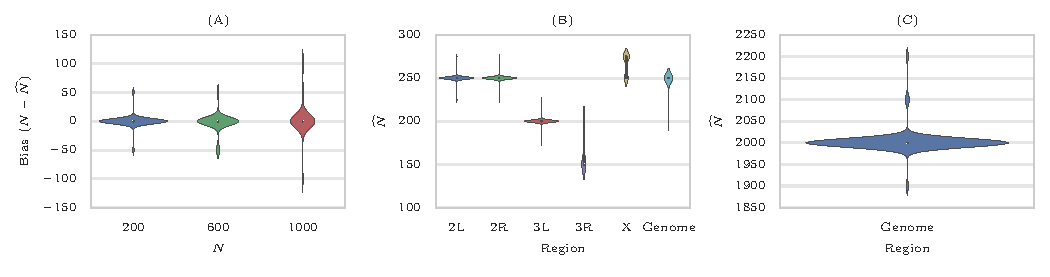
\includegraphics[width=\textwidth]{estimateNMLE.pdf}
	\caption{{\bf Estimating population size.}  (A) Distribution
		of bias in estimating $N$, computed on 1000 neutral
		simulations for each $N\in\{200,600,1000\}$ when $W=10$Mbp and 
		$r=2\times10^{-8}$. (B) 
		Estimates
		of population size for \datadm. For each case, the
		distribution of estimator is computed by 100 bootstrap
		computations using 1000 variants each. The multiple modes
		are an artifact of grid search used to speed up
		computation. (C) Distribution of the population 	size
		estimates on the yeast dataset.  Despite large census
		population size ($10^6-10^7$~\cite{burke2014standing}), this
		dataset exhibits much smaller effective population size
		($\hN=2000$). }
	\label{fig:estimateNMLE}
\end{figure*}

While it would be ideal to compute \comale\ statistic for each
replicate and chromosome separately, computing empirical $p$-values
and significant regions become computationally intensive as empirical
null distribution of each replicate and each chromosome needs to be
computed.  Hence, we use a single genome-wide estimate $\hN=250$ in
all analyses, but we normalize statistic $\Hc^*$ separately for each
chromosome.

We use a heuristic calculation (See~\ref{sec:winSize}) to choose the
sliding window size $L$ as the distance where the LD between the
favored mutation and a site $L/2$bp away remains strong. For \dmel
parameters, we obtained $L=30$Kbp. We computed the normalized test
statistic $\Hc^*$ on sliding windows of size of 30Kbp and step size of
5Kbp over the genome (See~\ref{fig:man-dmel-region}-A).

Empirical null distribution of $\Hc^*$ was estimated by creating 100
whole genome simulations (400K statistic values) as described in
Section~\ref{sec:sims}. Then, $p$-value of the test statistic in each
region in the experimental data was calculated as the fraction of the
null statistic values that are greater than or equal to the test
statistic(see~\ref{fig:null-alt}).  After correcting for multiple
testing, we identified $5$ contiguous
intervals~(\ref{fig:man-dmel-region}) satisfying FDR$\le0.05$, and
covering $2,829$ polymorphic sites. We further performed single-locus
hypothesis testing on the $2,829$ sites to identify $174$ individual
variants with FDR $\le0.01$~(\ref{fig:man-dmel-region}-B).

The final set of 174 variants fall within 32 genes(\ref{tab:genes})
including many Serine inhibitory proteases (serpins), and other genes
involved in endocytosis. Recycling of synaptic vesicles is seen to be
blocked at high temperature in temperature sensitive Drosophila
mutants~\cite{kosaka1983reversible}. This is also supported by GO
enrichment analysis, where a single GO term `inhibition of
proteolysis' is found to enriched (corrected $p$-value:0.0041).  To
test for dominant selection, we computed $D$ statistic on simulated
neutral and experimental data, and computed $p$-values accordingly.
After correcting for multiple testing, 96 variants were discovered
with FDR$\le 0.01$~(\ref{fig:man-dmel-snp}). 


\subsection{Analysis of Outcrossing Yeast Populations}
We also applied \comale\ to  $12$ replicate samples of
outcrossing yeast populations~\cite{burke2014standing}, where samples are 
taken at
generations $\Tc=\{0,180,360,540\}$. We observed a significant
variation in the genome-wide site frequency spectrum of certain
populations over different time points for some
replicates~(\ref{fig:yeast-sfs}). The variation does not have an
easily identifiable cause. Therefore, we focused analysis on seven
replicates $r\in\{3,7,8,9,10,11,12\}$ with genome-wide site-frequency
spectrum over the time range~(\ref{fig:yeast-pca}).

We estimated population size to be $\hN=2000$ haplotypes 
(\ref{fig:estimateNMLE}-C and \ref{fig:estimateN}-F), and computed
$\hs$, $\hh$ and $H$ statistic accordingly. To compute $p$-values, we
created 1M single-locus neutral simulations according to experimental
data's initial frequency and coverage. By setting FDR cutoff to
$0.05$, only 18 and 16 variants show significant signal for
directional and dominant selection,
respectively~(\ref{fig:man-dmel-snp}).  Selected variants for
directional selection are clustered in two regions, which match $2$ of
the $5$ regions (regions C and E in Fig. 2-a
in~\cite{burke2014standing}) identified by Burke~\emph{et al.} in
their preliminary analysis. 

\begin{figure*}
	\centering
	\begin{tabular}{c}
		(A)\\
		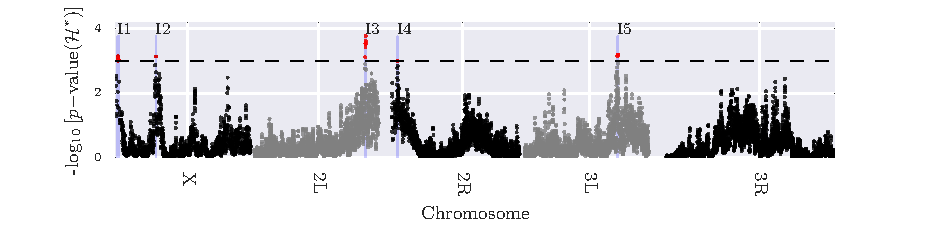
\includegraphics[trim=0.4in 0.in 0.6in 
		0in,clip,width=0.9\textwidth]{man-dmel-region.pdf}\\		
		(B)\\	
		\includegraphics[trim=0.3in 0.in 0.6in 
		.0in,clip,width=0.9\textwidth]{{topVariants.dmel.dir}.pdf}
	\end{tabular}
	\caption{{\bf Scan of \comale\ statistic on \datadm.}
		(A)         Manhattan plot of scan for $\Hc^*$ statistic using sliding 
		window of 
		size $L=3000$ over the
		genome.  The dashed line represents cutoff for genome-wide
		FDR$\le0.05$, and identifies 5 contiguous intervals, I1-I5, 
		which are shaded in blue. (B) Trajectories of the selected 
		variants within 
		intervals I1-I5.}
	\label{fig:man-dmel-region}
\end{figure*}



\begin{figure*}
	\centering
	\begin{tabular}{cc}
		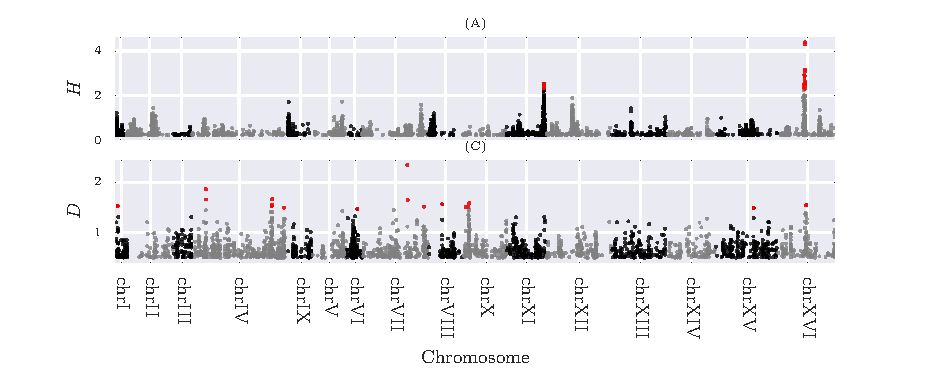
\includegraphics[trim=0.4in 0.in 0.6in 
		0.0in,clip,width=0.65\textwidth]{man-yeast-snp.pdf}&	
		\raisebox{0.2in}{
			\includegraphics[trim=0in 0.in 0in 
			0.0in,clip,width=0.35\textwidth]{{topVariants.yeast}.pdf}}
	\end{tabular}
	\caption{{\bf Single locus analysis of the yeast outcrossing 
			populations.}\\ Manhattan plot 
		of scan single locus \comale\ statistic ($L=1$) for testing directional 
		selection (A) and dominant 
		selection 
		(C).
		The dashed line represents cutoff for  genome-wide FDR$\le0.05$.
		Trajectories of the selected variants are depicted in panels (B) and 
		(D).}
	\label{fig:man-yeast-snp}
\end{figure*}



